\documentclass{standalone}
\usepackage{tikz}
\usetikzlibrary{patterns, positioning}
\usepackage[sfdefault]{ClearSans} %% option 'sfdefault' activates Clear Sans as the default text font
\usepackage[T1]{fontenc}

\begin{document}
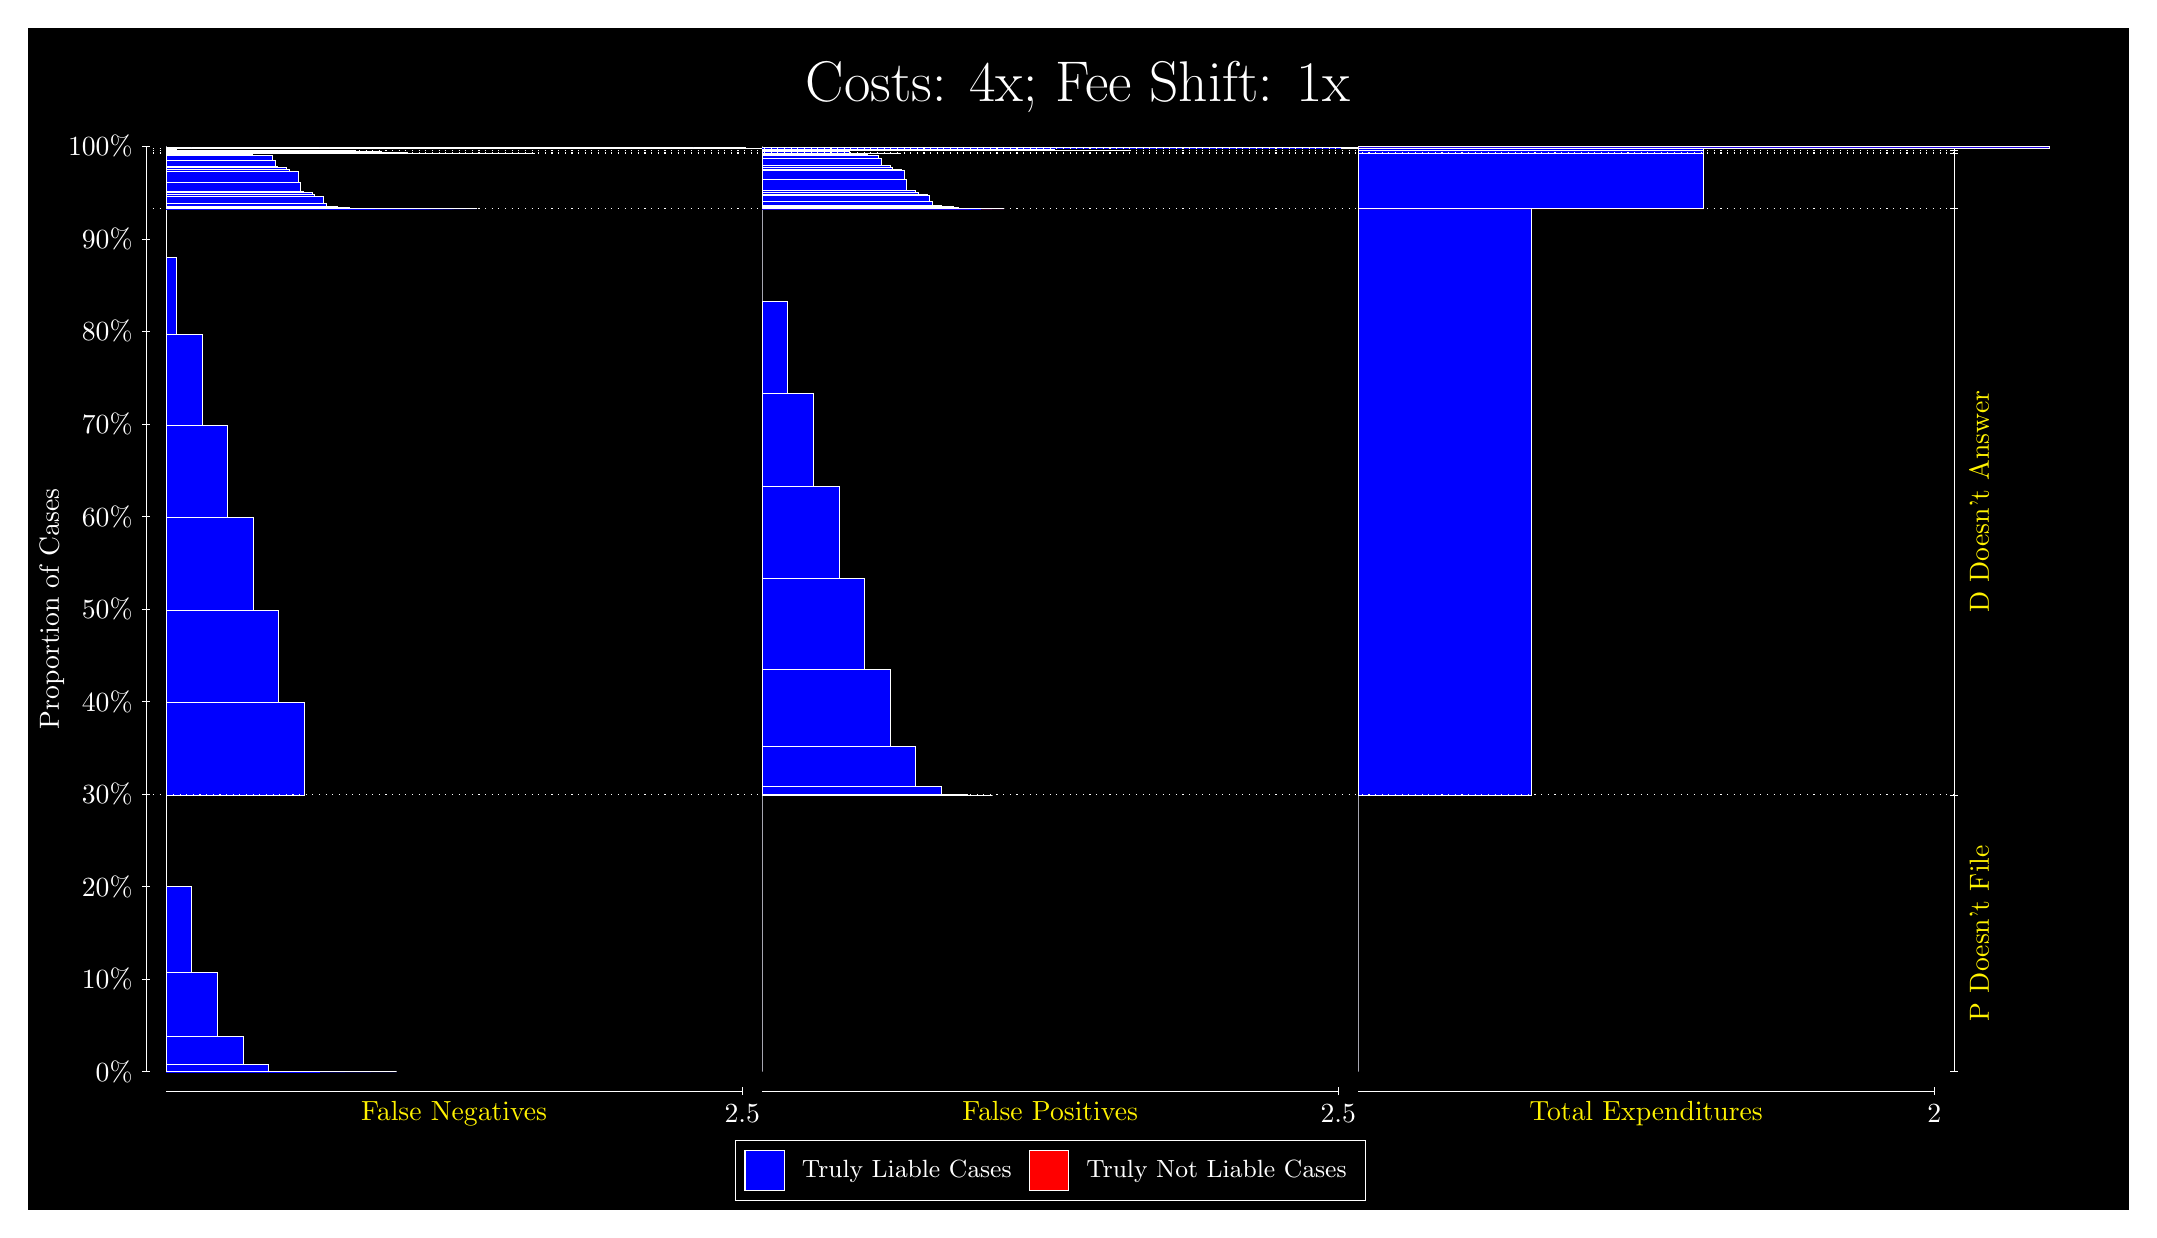
\begin{tikzpicture}
\draw[fill=black] (0,0) rectangle (26.667,15);
\draw[text=white] (0,13.5) rectangle (26.667,15) node[midway] {\huge Costs: 4x; Fee Shift: 1x};
\draw[white, very thin] (1.5,1.75) -- (1.5,13.5);
\node[rotate=90, text=white, anchor=center] at (0.3, 7.625) {Proportion of Cases};
\draw[white, very thin] (1.45,1.75) -- (1.55,1.75);
\node[text=white, anchor=east] at (1.45, 1.75) {0\%};
\draw[white, very thin] (1.45,2.925) -- (1.55,2.925);
\node[text=white, anchor=east] at (1.45, 2.925) {10\%};
\draw[white, very thin] (1.45,4.1) -- (1.55,4.1);
\node[text=white, anchor=east] at (1.45, 4.1) {20\%};
\draw[white, very thin] (1.45,5.275) -- (1.55,5.275);
\node[text=white, anchor=east] at (1.45, 5.275) {30\%};
\draw[white, very thin] (1.45,6.45) -- (1.55,6.45);
\node[text=white, anchor=east] at (1.45, 6.45) {40\%};
\draw[white, very thin] (1.45,7.625) -- (1.55,7.625);
\node[text=white, anchor=east] at (1.45, 7.625) {50\%};
\draw[white, very thin] (1.45,8.8) -- (1.55,8.8);
\node[text=white, anchor=east] at (1.45, 8.8) {60\%};
\draw[white, very thin] (1.45,9.975) -- (1.55,9.975);
\node[text=white, anchor=east] at (1.45, 9.975) {70\%};
\draw[white, very thin] (1.45,11.15) -- (1.55,11.15);
\node[text=white, anchor=east] at (1.45, 11.15) {80\%};
\draw[white, very thin] (1.45,12.325) -- (1.55,12.325);
\node[text=white, anchor=east] at (1.45, 12.325) {90\%};
\draw[white, very thin] (1.45,13.5) -- (1.55,13.5);
\node[text=white, anchor=east] at (1.45, 13.5) {100\%};

\draw[white, very thin] (24.457,1.75) -- (24.457,13.5);
\draw[white, very thin] (24.407,1.75) -- (24.507,1.75);
\node[anchor=west] at (24.407, 1.75) {};
\draw[white, very thin] (24.407,5.264) -- (24.507,5.264);
\node[anchor=west] at (24.407, 5.264) {};
\draw[white, very thin] (24.407,12.709) -- (24.507,12.709);
\node[anchor=west] at (24.407, 12.709) {};
\draw[white, very thin] (24.407,13.415) -- (24.507,13.415);
\node[anchor=west] at (24.407, 13.415) {};
\draw[white, very thin] (24.407,13.451) -- (24.507,13.451);
\node[anchor=west] at (24.407, 13.451) {};
\draw[white, very thin] (24.407,13.478) -- (24.507,13.478);
\node[anchor=west] at (24.407, 13.478) {};
\draw[white, very thin] (24.407,13.5) -- (24.507,13.5);
\node[anchor=west] at (24.407, 13.5) {};

\draw[white, very thin, fill=blue] (1.75,1.75) rectangle (4.6775,1.75);
\draw[white, very thin, fill=blue] (1.75,1.75) rectangle (4.3523,1.75);
\draw[white, very thin, fill=blue] (1.75,1.75) rectangle (4.027,1.75);
\draw[white, very thin, fill=blue] (1.75,1.75) rectangle (3.7017,1.7503);
\draw[white, very thin, fill=blue] (1.75,1.7503) rectangle (3.3764,1.7576);
\draw[white, very thin, fill=blue] (1.75,1.7576) rectangle (3.0511,1.8361);
\draw[white, very thin, fill=blue] (1.75,1.8361) rectangle (2.7258,2.1984);
\draw[white, very thin, fill=blue] (1.75,2.1984) rectangle (2.4006,3.0086);
\draw[white, very thin, fill=blue] (1.75,3.0086) rectangle (2.0753,4.0995);
\draw[white, very thin, fill=red] (1.75,4.0995) rectangle (1.75,4.0995);
\draw[white, very thin, fill=blue] (1.75,4.0995) rectangle (1.75,5.264);
\draw[white, very thin, fill=blue] (1.75,5.264) rectangle (3.5065,6.439);
\draw[white, very thin, fill=blue] (1.75,6.439) rectangle (3.1812,7.614);
\draw[white, very thin, fill=blue] (1.75,7.614) rectangle (2.856,8.7889);
\draw[white, very thin, fill=blue] (1.75,8.7889) rectangle (2.5307,9.9623);
\draw[white, very thin, fill=blue] (1.75,9.9623) rectangle (2.2054,11.111);
\draw[white, very thin, fill=blue] (1.75,11.111) rectangle (1.8801,12.093);
\draw[white, very thin, fill=red] (1.75,12.093) rectangle (1.75,12.093);
\draw[white, very thin, fill=blue] (1.75,12.093) rectangle (1.75,12.709);
\draw[white, very thin, fill=blue] (1.75,12.709) rectangle (5.7022,12.709);
\draw[white, very thin, fill=blue] (1.75,12.709) rectangle (5.5558,12.709);
\draw[white, very thin, fill=blue] (1.75,12.709) rectangle (5.4094,12.709);
\draw[white, very thin, fill=blue] (1.75,12.709) rectangle (5.3769,12.709);
\draw[white, very thin, fill=blue] (1.75,12.709) rectangle (5.2631,12.709);
\draw[white, very thin, fill=blue] (1.75,12.709) rectangle (5.2305,12.709);
\draw[white, very thin, fill=blue] (1.75,12.709) rectangle (5.1167,12.709);
\draw[white, very thin, fill=blue] (1.75,12.709) rectangle (5.0842,12.709);
\draw[white, very thin, fill=blue] (1.75,12.709) rectangle (5.0516,12.709);
\draw[white, very thin, fill=blue] (1.75,12.709) rectangle (4.9378,12.709);
\draw[white, very thin, fill=blue] (1.75,12.709) rectangle (4.9052,12.709);
\draw[white, very thin, fill=blue] (1.75,12.709) rectangle (4.7914,12.709);
\draw[white, very thin, fill=blue] (1.75,12.709) rectangle (4.7589,12.709);
\draw[white, very thin, fill=blue] (1.75,12.709) rectangle (4.7263,12.709);
\draw[white, very thin, fill=blue] (1.75,12.709) rectangle (4.6125,12.709);
\draw[white, very thin, fill=blue] (1.75,12.709) rectangle (4.58,12.709);
\draw[white, very thin, fill=blue] (1.75,12.709) rectangle (4.4661,12.709);
\draw[white, very thin, fill=blue] (1.75,12.709) rectangle (4.4336,12.709);
\draw[white, very thin, fill=blue] (1.75,12.709) rectangle (4.4011,12.71);
\draw[white, very thin, fill=blue] (1.75,12.71) rectangle (4.2872,12.71);
\draw[white, very thin, fill=blue] (1.75,12.71) rectangle (4.2547,12.71);
\draw[white, very thin, fill=blue] (1.75,12.71) rectangle (4.1408,12.711);
\draw[white, very thin, fill=blue] (1.75,12.711) rectangle (4.1083,12.714);
\draw[white, very thin, fill=blue] (1.75,12.714) rectangle (4.0758,12.728);
\draw[white, very thin, fill=blue] (1.75,12.728) rectangle (3.9619,12.731);
\draw[white, very thin, fill=blue] (1.75,12.731) rectangle (3.9294,12.736);
\draw[white, very thin, fill=blue] (1.75,12.736) rectangle (3.8155,12.742);
\draw[white, very thin, fill=blue] (1.75,12.742) rectangle (3.783,12.78);
\draw[white, very thin, fill=blue] (1.75,12.78) rectangle (3.7505,12.869);
\draw[white, very thin, fill=blue] (1.75,12.869) rectangle (3.6366,12.887);
\draw[white, very thin, fill=blue] (1.75,12.887) rectangle (3.6041,12.911);
\draw[white, very thin, fill=blue] (1.75,12.911) rectangle (3.4903,12.93);
\draw[white, very thin, fill=blue] (1.75,12.93) rectangle (3.4577,13.044);
\draw[white, very thin, fill=blue] (1.75,13.044) rectangle (3.4252,13.184);
\draw[white, very thin, fill=blue] (1.75,13.184) rectangle (3.3114,13.21);
\draw[white, very thin, fill=blue] (1.75,13.21) rectangle (3.2788,13.23);
\draw[white, very thin, fill=blue] (1.75,13.23) rectangle (3.165,13.243);
\draw[white, very thin, fill=blue] (1.75,13.243) rectangle (3.1325,13.32);
\draw[white, very thin, fill=blue] (1.75,13.32) rectangle (3.0999,13.38);
\draw[white, very thin, fill=blue] (1.75,13.38) rectangle (2.9861,13.388);
\draw[white, very thin, fill=blue] (1.75,13.388) rectangle (2.9535,13.391);
\draw[white, very thin, fill=blue] (1.75,13.391) rectangle (2.8397,13.393);
\draw[white, very thin, fill=blue] (1.75,13.393) rectangle (2.8072,13.405);
\draw[white, very thin, fill=blue] (1.75,13.405) rectangle (2.7746,13.414);
\draw[white, very thin, fill=blue] (1.75,13.414) rectangle (2.6608,13.415);
\draw[white, very thin, fill=blue] (1.75,13.415) rectangle (2.6283,13.415);
\draw[white, very thin, fill=blue] (1.75,13.415) rectangle (2.5144,13.415);
\draw[white, very thin, fill=blue] (1.75,13.415) rectangle (2.4819,13.415);
\draw[white, very thin, fill=blue] (1.75,13.415) rectangle (2.3355,13.415);
\draw[white, very thin, fill=blue] (1.75,13.415) rectangle (2.1891,13.415);
\draw[white, very thin, fill=red] (1.75,13.415) rectangle (1.75,13.415);
\draw[white, very thin, fill=blue] (1.75,13.415) rectangle (6.4341,13.415);
\draw[white, very thin, fill=blue] (1.75,13.415) rectangle (6.1088,13.415);
\draw[white, very thin, fill=blue] (1.75,13.415) rectangle (5.7835,13.415);
\draw[white, very thin, fill=blue] (1.75,13.415) rectangle (5.4582,13.415);
\draw[white, very thin, fill=blue] (1.75,13.415) rectangle (5.1329,13.416);
\draw[white, very thin, fill=blue] (1.75,13.416) rectangle (4.8077,13.42);
\draw[white, very thin, fill=blue] (1.75,13.42) rectangle (4.4824,13.436);
\draw[white, very thin, fill=blue] (1.75,13.436) rectangle (4.1571,13.449);
\draw[white, very thin, fill=blue] (1.75,13.449) rectangle (3.8318,13.451);
\draw[white, very thin, fill=blue] (1.75,13.451) rectangle (3.5065,13.451);
\draw[white, very thin, fill=red] (1.75,13.451) rectangle (1.75,13.451);
\draw[white, very thin, fill=blue] (1.75,13.451) rectangle (3.5065,13.451);
\draw[white, very thin, fill=blue] (1.75,13.451) rectangle (3.1812,13.451);
\draw[white, very thin, fill=blue] (1.75,13.451) rectangle (2.856,13.451);
\draw[white, very thin, fill=blue] (1.75,13.451) rectangle (2.5307,13.452);
\draw[white, very thin, fill=blue] (1.75,13.452) rectangle (2.2054,13.455);
\draw[white, very thin, fill=blue] (1.75,13.455) rectangle (1.8801,13.465);
\draw[white, very thin, fill=red] (1.75,13.465) rectangle (1.75,13.465);
\draw[white, very thin, fill=blue] (1.75,13.465) rectangle (1.75,13.478);
\draw[white, very thin, fill=blue] (1.75,13.478) rectangle (11.704,13.478);
\draw[white, very thin, fill=blue] (1.75,13.478) rectangle (11.378,13.478);
\draw[white, very thin, fill=blue] (1.75,13.478) rectangle (11.053,13.478);
\draw[white, very thin, fill=blue] (1.75,13.478) rectangle (10.728,13.478);
\draw[white, very thin, fill=blue] (1.75,13.478) rectangle (10.403,13.478);
\draw[white, very thin, fill=blue] (1.75,13.478) rectangle (10.403,13.478);
\draw[white, very thin, fill=blue] (1.75,13.478) rectangle (10.077,13.478);
\draw[white, very thin, fill=blue] (1.75,13.478) rectangle (9.752,13.479);
\draw[white, very thin, fill=blue] (1.75,13.479) rectangle (9.752,13.479);
\draw[white, very thin, fill=blue] (1.75,13.479) rectangle (9.4267,13.48);
\draw[white, very thin, fill=blue] (1.75,13.48) rectangle (9.4267,13.481);
\draw[white, very thin, fill=blue] (1.75,13.481) rectangle (9.1014,13.485);
\draw[white, very thin, fill=blue] (1.75,13.485) rectangle (8.7761,13.487);
\draw[white, very thin, fill=blue] (1.75,13.487) rectangle (8.4508,13.487);
\draw[white, very thin, fill=blue] (1.75,13.487) rectangle (8.1255,13.487);
\draw[white, very thin, fill=blue] (1.75,13.487) rectangle (7.8003,13.487);
\draw[white, very thin, fill=blue] (1.75,13.487) rectangle (7.475,13.487);
\draw[white, very thin, fill=blue] (1.75,13.487) rectangle (3.7017,13.487);
\draw[white, very thin, fill=blue] (1.75,13.487) rectangle (3.3764,13.487);
\draw[white, very thin, fill=blue] (1.75,13.487) rectangle (3.0511,13.487);
\draw[white, very thin, fill=blue] (1.75,13.487) rectangle (3.0511,13.487);
\draw[white, very thin, fill=blue] (1.75,13.487) rectangle (2.7258,13.487);
\draw[white, very thin, fill=blue] (1.75,13.487) rectangle (2.7258,13.487);
\draw[white, very thin, fill=blue] (1.75,13.487) rectangle (2.7258,13.487);
\draw[white, very thin, fill=blue] (1.75,13.487) rectangle (2.4006,13.487);
\draw[white, very thin, fill=blue] (1.75,13.487) rectangle (2.4006,13.487);
\draw[white, very thin, fill=blue] (1.75,13.487) rectangle (2.0753,13.487);
\draw[white, very thin, fill=blue] (1.75,13.487) rectangle (2.0753,13.488);
\draw[white, very thin, fill=blue] (1.75,13.488) rectangle (2.0753,13.488);
\draw[white, very thin, fill=red] (1.75,13.488) rectangle (1.75,13.488);
\draw[white, very thin, fill=blue] (1.75,13.488) rectangle (1.75,13.5);
\draw[white, very thin, fill=red] (9.3189,1.75) rectangle (9.3189,1.75);
\draw[white, very thin, fill=blue] (9.3189,1.75) rectangle (9.3189,5.264);
\draw[white, very thin, fill=red] (9.3189,5.264) rectangle (12.246,5.264);
\draw[white, very thin, fill=blue] (9.3189,5.264) rectangle (12.246,5.264);
\draw[white, very thin, fill=blue] (9.3189,5.264) rectangle (11.921,5.2692);
\draw[white, very thin, fill=blue] (9.3189,5.2692) rectangle (11.596,5.3683);
\draw[white, very thin, fill=blue] (9.3189,5.3683) rectangle (11.271,5.8808);
\draw[white, very thin, fill=blue] (9.3189,5.8808) rectangle (10.945,6.8619);
\draw[white, very thin, fill=blue] (9.3189,6.8619) rectangle (10.62,8.0111);
\draw[white, very thin, fill=blue] (9.3189,8.0111) rectangle (10.295,9.1844);
\draw[white, very thin, fill=blue] (9.3189,9.1844) rectangle (9.9694,10.359);
\draw[white, very thin, fill=blue] (9.3189,10.359) rectangle (9.6442,11.534);
\draw[white, very thin, fill=blue] (9.3189,11.534) rectangle (9.3189,12.709);
\draw[white, very thin, fill=red] (9.3189,12.709) rectangle (12.393,12.709);
\draw[white, very thin, fill=blue] (9.3189,12.709) rectangle (12.393,12.709);
\draw[white, very thin, fill=red] (9.3189,12.709) rectangle (12.246,12.709);
\draw[white, very thin, fill=blue] (9.3189,12.709) rectangle (12.246,12.709);
\draw[white, very thin, fill=red] (9.3189,12.709) rectangle (12.1,12.709);
\draw[white, very thin, fill=blue] (9.3189,12.709) rectangle (12.1,12.71);
\draw[white, very thin, fill=blue] (9.3189,12.71) rectangle (12.068,12.71);
\draw[white, very thin, fill=red] (9.3189,12.71) rectangle (11.954,12.71);
\draw[white, very thin, fill=blue] (9.3189,12.71) rectangle (11.954,12.71);
\draw[white, very thin, fill=blue] (9.3189,12.71) rectangle (11.921,12.711);
\draw[white, very thin, fill=red] (9.3189,12.711) rectangle (11.807,12.711);
\draw[white, very thin, fill=blue] (9.3189,12.711) rectangle (11.807,12.72);
\draw[white, very thin, fill=blue] (9.3189,12.72) rectangle (11.775,12.732);
\draw[white, very thin, fill=blue] (9.3189,12.732) rectangle (11.742,12.734);
\draw[white, very thin, fill=blue] (9.3189,12.734) rectangle (11.628,12.737);
\draw[white, very thin, fill=blue] (9.3189,12.737) rectangle (11.596,12.745);
\draw[white, very thin, fill=blue] (9.3189,12.745) rectangle (11.482,12.805);
\draw[white, very thin, fill=blue] (9.3189,12.805) rectangle (11.449,12.882);
\draw[white, very thin, fill=blue] (9.3189,12.882) rectangle (11.417,12.895);
\draw[white, very thin, fill=blue] (9.3189,12.895) rectangle (11.303,12.915);
\draw[white, very thin, fill=blue] (9.3189,12.915) rectangle (11.271,12.941);
\draw[white, very thin, fill=blue] (9.3189,12.941) rectangle (11.157,13.081);
\draw[white, very thin, fill=blue] (9.3189,13.081) rectangle (11.124,13.195);
\draw[white, very thin, fill=blue] (9.3189,13.195) rectangle (11.092,13.214);
\draw[white, very thin, fill=blue] (9.3189,13.214) rectangle (10.978,13.238);
\draw[white, very thin, fill=blue] (9.3189,13.238) rectangle (10.945,13.256);
\draw[white, very thin, fill=blue] (9.3189,13.256) rectangle (10.831,13.344);
\draw[white, very thin, fill=blue] (9.3189,13.344) rectangle (10.799,13.383);
\draw[white, very thin, fill=blue] (9.3189,13.383) rectangle (10.766,13.389);
\draw[white, very thin, fill=blue] (9.3189,13.389) rectangle (10.653,13.394);
\draw[white, very thin, fill=blue] (9.3189,13.394) rectangle (10.62,13.397);
\draw[white, very thin, fill=blue] (9.3189,13.397) rectangle (10.506,13.411);
\draw[white, very thin, fill=blue] (9.3189,13.411) rectangle (10.474,13.414);
\draw[white, very thin, fill=blue] (9.3189,13.414) rectangle (10.441,13.415);
\draw[white, very thin, fill=blue] (9.3189,13.415) rectangle (10.327,13.415);
\draw[white, very thin, fill=blue] (9.3189,13.415) rectangle (10.295,13.415);
\draw[white, very thin, fill=blue] (9.3189,13.415) rectangle (10.181,13.415);
\draw[white, very thin, fill=blue] (9.3189,13.415) rectangle (10.148,13.415);
\draw[white, very thin, fill=blue] (9.3189,13.415) rectangle (10.116,13.415);
\draw[white, very thin, fill=blue] (9.3189,13.415) rectangle (10.002,13.415);
\draw[white, very thin, fill=blue] (9.3189,13.415) rectangle (9.9694,13.415);
\draw[white, very thin, fill=blue] (9.3189,13.415) rectangle (9.8556,13.415);
\draw[white, very thin, fill=blue] (9.3189,13.415) rectangle (9.8231,13.415);
\draw[white, very thin, fill=blue] (9.3189,13.415) rectangle (9.7905,13.415);
\draw[white, very thin, fill=blue] (9.3189,13.415) rectangle (9.6767,13.415);
\draw[white, very thin, fill=blue] (9.3189,13.415) rectangle (9.6442,13.415);
\draw[white, very thin, fill=blue] (9.3189,13.415) rectangle (9.5303,13.415);
\draw[white, very thin, fill=blue] (9.3189,13.415) rectangle (9.4978,13.415);
\draw[white, very thin, fill=blue] (9.3189,13.415) rectangle (9.4652,13.415);
\draw[white, very thin, fill=blue] (9.3189,13.415) rectangle (9.3514,13.415);
\draw[white, very thin, fill=blue] (9.3189,13.415) rectangle (9.3189,13.415);
\draw[white, very thin, fill=red] (9.3189,13.415) rectangle (11.075,13.415);
\draw[white, very thin, fill=blue] (9.3189,13.415) rectangle (11.075,13.416);
\draw[white, very thin, fill=blue] (9.3189,13.416) rectangle (10.75,13.418);
\draw[white, very thin, fill=blue] (9.3189,13.418) rectangle (10.425,13.431);
\draw[white, very thin, fill=blue] (9.3189,13.431) rectangle (10.1,13.447);
\draw[white, very thin, fill=blue] (9.3189,13.447) rectangle (9.7743,13.451);
\draw[white, very thin, fill=blue] (9.3189,13.451) rectangle (9.449,13.451);
\draw[white, very thin, fill=blue] (9.3189,13.451) rectangle (9.3189,13.451);
\draw[white, very thin, fill=red] (9.3189,13.451) rectangle (14.003,13.451);
\draw[white, very thin, fill=blue] (9.3189,13.451) rectangle (14.003,13.451);
\draw[white, very thin, fill=blue] (9.3189,13.451) rectangle (13.678,13.451);
\draw[white, very thin, fill=blue] (9.3189,13.451) rectangle (13.352,13.454);
\draw[white, very thin, fill=blue] (9.3189,13.454) rectangle (13.027,13.464);
\draw[white, very thin, fill=blue] (9.3189,13.464) rectangle (12.702,13.474);
\draw[white, very thin, fill=blue] (9.3189,13.474) rectangle (12.377,13.477);
\draw[white, very thin, fill=blue] (9.3189,13.477) rectangle (12.051,13.478);
\draw[white, very thin, fill=blue] (9.3189,13.478) rectangle (11.726,13.478);
\draw[white, very thin, fill=blue] (9.3189,13.478) rectangle (11.401,13.478);
\draw[white, very thin, fill=blue] (9.3189,13.478) rectangle (11.075,13.478);
\draw[white, very thin, fill=red] (9.3189,13.478) rectangle (19.273,13.478);
\draw[white, very thin, fill=blue] (9.3189,13.478) rectangle (19.273,13.478);
\draw[white, very thin, fill=red] (9.3189,13.478) rectangle (18.947,13.478);
\draw[white, very thin, fill=blue] (9.3189,13.478) rectangle (18.947,13.478);
\draw[white, very thin, fill=red] (9.3189,13.478) rectangle (18.622,13.478);
\draw[white, very thin, fill=blue] (9.3189,13.478) rectangle (18.622,13.478);
\draw[white, very thin, fill=red] (9.3189,13.478) rectangle (18.297,13.478);
\draw[white, very thin, fill=blue] (9.3189,13.478) rectangle (18.297,13.478);
\draw[white, very thin, fill=red] (9.3189,13.478) rectangle (17.971,13.478);
\draw[white, very thin, fill=blue] (9.3189,13.478) rectangle (17.971,13.478);
\draw[white, very thin, fill=blue] (9.3189,13.478) rectangle (17.971,13.478);
\draw[white, very thin, fill=blue] (9.3189,13.478) rectangle (17.646,13.478);
\draw[white, very thin, fill=red] (9.3189,13.478) rectangle (17.646,13.478);
\draw[white, very thin, fill=blue] (9.3189,13.478) rectangle (17.646,13.478);
\draw[white, very thin, fill=red] (9.3189,13.478) rectangle (17.321,13.478);
\draw[white, very thin, fill=blue] (9.3189,13.478) rectangle (17.321,13.479);
\draw[white, very thin, fill=blue] (9.3189,13.479) rectangle (17.321,13.479);
\draw[white, very thin, fill=blue] (9.3189,13.479) rectangle (16.996,13.48);
\draw[white, very thin, fill=blue] (9.3189,13.48) rectangle (16.996,13.482);
\draw[white, very thin, fill=blue] (9.3189,13.482) rectangle (16.67,13.484);
\draw[white, very thin, fill=blue] (9.3189,13.484) rectangle (16.67,13.486);
\draw[white, very thin, fill=blue] (9.3189,13.486) rectangle (16.345,13.487);
\draw[white, very thin, fill=blue] (9.3189,13.487) rectangle (16.345,13.488);
\draw[white, very thin, fill=blue] (9.3189,13.488) rectangle (16.345,13.49);
\draw[white, very thin, fill=blue] (9.3189,13.49) rectangle (16.02,13.49);
\draw[white, very thin, fill=blue] (9.3189,13.49) rectangle (16.02,13.491);
\draw[white, very thin, fill=blue] (9.3189,13.491) rectangle (15.694,13.491);
\draw[white, very thin, fill=blue] (9.3189,13.491) rectangle (15.694,13.491);
\draw[white, very thin, fill=blue] (9.3189,13.491) rectangle (15.369,13.491);
\draw[white, very thin, fill=blue] (9.3189,13.491) rectangle (15.369,13.491);
\draw[white, very thin, fill=blue] (9.3189,13.491) rectangle (15.044,13.491);
\draw[white, very thin, fill=blue] (9.3189,13.491) rectangle (15.044,13.491);
\draw[white, very thin, fill=blue] (9.3189,13.491) rectangle (14.719,13.491);
\draw[white, very thin, fill=blue] (9.3189,13.491) rectangle (14.719,13.491);
\draw[white, very thin, fill=blue] (9.3189,13.491) rectangle (14.393,13.491);
\draw[white, very thin, fill=red] (9.3189,13.491) rectangle (10.62,13.491);
\draw[white, very thin, fill=blue] (9.3189,13.491) rectangle (10.62,13.491);
\draw[white, very thin, fill=red] (9.3189,13.491) rectangle (10.295,13.491);
\draw[white, very thin, fill=blue] (9.3189,13.491) rectangle (10.295,13.491);
\draw[white, very thin, fill=red] (9.3189,13.491) rectangle (9.9694,13.491);
\draw[white, very thin, fill=blue] (9.3189,13.491) rectangle (9.9694,13.491);
\draw[white, very thin, fill=red] (9.3189,13.491) rectangle (9.6442,13.491);
\draw[white, very thin, fill=blue] (9.3189,13.491) rectangle (9.6442,13.491);
\draw[white, very thin, fill=red] (9.3189,13.491) rectangle (9.3189,13.491);
\draw[white, very thin, fill=blue] (9.3189,13.491) rectangle (9.3189,13.5);
\draw[white, very thin, fill=red] (16.888,1.75) rectangle (16.888,1.75);
\draw[white, very thin, fill=blue] (16.888,1.75) rectangle (16.888,5.264);
\draw[white, very thin, fill=red] (16.888,5.264) rectangle (19.083,5.264);
\draw[white, very thin, fill=blue] (16.888,5.264) rectangle (19.083,12.709);
\draw[white, very thin, fill=red] (16.888,12.709) rectangle (21.279,12.709);
\draw[white, very thin, fill=blue] (16.888,12.709) rectangle (21.279,13.415);
\draw[white, very thin, fill=red] (16.888,13.415) rectangle (21.279,13.415);
\draw[white, very thin, fill=blue] (16.888,13.415) rectangle (21.279,13.451);
\draw[white, very thin, fill=red] (16.888,13.451) rectangle (21.279,13.451);
\draw[white, very thin, fill=blue] (16.888,13.451) rectangle (21.279,13.478);
\draw[white, very thin, fill=red] (16.888,13.478) rectangle (25.67,13.478);
\draw[white, very thin, fill=blue] (16.888,13.478) rectangle (25.67,13.481);
\draw[white, very thin, fill=red] (16.888,13.481) rectangle (25.67,13.481);
\draw[white, very thin, fill=blue] (16.888,13.481) rectangle (25.67,13.496);
\draw[white, very thin, fill=red] (16.888,13.496) rectangle (25.67,13.496);
\draw[white, very thin, fill=blue] (16.888,13.496) rectangle (25.67,13.5);
\draw[white, dotted] (1.5,5.264) -- (24.457,5.264);
\draw[white, dotted] (1.5,12.709) -- (24.457,12.709);
\draw[white, dotted] (1.5,13.415) -- (24.457,13.415);
\draw[white, dotted] (1.5,13.451) -- (24.457,13.451);
\draw[white, dotted] (1.5,13.478) -- (24.457,13.478);
\draw[white, very thin] (1.75,1.5) -- (9.0689,1.5);
\node[text=yellow, anchor=north] at (5.4094, 1.5) {False Negatives};
\draw[white, very thin] (9.0689,1.45) -- (9.0689,1.55);
\node[text=white, anchor=north] at (9.0689, 1.45) {2.5};

\draw[white, very thin] (9.3189,1.5) -- (16.638,1.5);
\node[text=yellow, anchor=north] at (12.978, 1.5) {False Positives};
\draw[white, very thin] (16.638,1.45) -- (16.638,1.55);
\node[text=white, anchor=north] at (16.638, 1.45) {2.5};

\draw[white, very thin] (16.888,1.5) -- (24.207,1.5);
\node[text=yellow, anchor=north] at (20.547, 1.5) {Total Expenditures};
\draw[white, very thin] (24.207,1.45) -- (24.207,1.55);
\node[text=white, anchor=north] at (24.207, 1.45) {2};

\node[text=yellow, centered, rotate=90] at (24.777, 3.507) {P Doesn't File};
\node[text=yellow, centered, rotate=90] at (24.777, 8.9867) {D Doesn't Answer};





\draw (12.978300999999998,1.5) node[draw=none] (baseCoordinate) {};
\begin{scope}[align=center]
        \matrix[scale=0.5, draw=white, below=0.5cm of baseCoordinate, nodes={draw}, column sep=0.1cm]{
            \node[rectangle, draw, minimum width=0.5cm, minimum height=0.5cm, fill=blue] {}; &
            \node[draw=none, font=\small, text=white] (B) {Truly Liable Cases}; &
            \node[rectangle, draw, minimum width=0.5cm, minimum height=0.5cm, fill=red] {}; &
            \node[draw=none, font=\small, text=white] (B) {Truly Not Liable Cases}; \\
            };
\end{scope}

\end{tikzpicture}
\end{document}